\documentclass[11pt, oneside]{article} %Use "amsart" instead of "article" for AMSLaTeX format

\usepackage[left=2cm,top=3cm,right=2cm,bottom=4cm,head=1cm,a4paper]{geometry}    
\usepackage[utf8]{inputenc}
\usepackage{graphicx} %Use pdf, png, jpg, or eps§ with pdflatex; use eps in DVI mode
\usepackage{graphicx}
\usepackage{amsmath}
\usepackage{amssymb}
\usepackage{hyperref}
\usepackage{soul}
\usepackage{dsfont}
\usepackage{enumitem}
\usepackage{amsmath}
\usepackage{multicol}
\usepackage{amssymb}
\usepackage{braket}
\numberwithin{equation}{section}
\usepackage{bm}
\usepackage{appendix}
\usepackage{microtype}
\usepackage[nobottomtitles*]{titlesec}
\usepackage{hyperref}
\usepackage{subfiles}
\usepackage{bbm}
\hypersetup{
    colorlinks,
    citecolor=black,
    filecolor=black,
    linkcolor=black,
    urlcolor=black
}

%Tikz stuff:
\usepackage{tikz}
\usetikzlibrary{decorations.markings}
\usetikzlibrary{arrows,positioning} 
%\usepackage{pgfplots}

\newcommand{\noteAG}[1]{{\color[rgb]{0.,0.,0.8}[AG: #1]}}
\newcommand{\addAG}[1]{{\color[rgb]{0.,0.,0.8}{#1}}}

% math commands:
\newcommand*{\vertbar}{\rule[-1ex]{0.5pt}{2.5ex}}
\newcommand*{\horzbar}{\rule[.5ex]{2.5ex}{0.5pt}}
\newcommand{\dline}[1]{\underline{\underline{#1}}}

\newcommand{\inner}[1]{\left \langle #1  \right \rangle}
\newcommand{\sgn}{\textup{sgn}}
\newcommand{\tr}{\ensuremath{\textup{Tr}}}
\newcommand{\1}{\ensuremath{\mathbbm{1}}}
\newcommand{\re}{\ensuremath{\textup{Re}}}
\newcommand{\im}{\ensuremath{\textup{Im}}}
\newcommand{\ts}{\textsuperscript}
\renewcommand{\r}{\ensuremath{\textbf{r}}}
\newcommand{\jon} {J_{\textup{on}}}
\newcommand{\joff} {J_{\textup{off}}}
\newcommand{\ketbra}[2]{\ket{#1}\!\bra{#2}}
\newcommand{\qkit}{\mathcal Q_{\textup{Kit}}}
\newcommand{\ujk}{u_{jk}}
\newcommand{\pdag}{\phantom{\dag}}
\renewcommand{\thefootnote}{\roman{footnote}}
\newcommand{\loctr}{\textup{tr}}
\newcommand{\egs}{E_\textup{g.s.}}

\newcommand{\normord}[1]{:\mathrel{#1}:}

\newcommand{\peru}[1]{{\color[rgb]{0.,0.,0.8}[\textbf{Peru: #1]}}}
\newcommand{\justin}[1]{{\color[rgb]{1,0.2,0.}[\textbf{Justin: #1]}}}


%Define that shaded box you like
\usepackage[noframe]{showframe}
\usepackage{framed}
\renewenvironment{shaded}{%
    \everypar={{\setbox0=\lastbox}\everypar{}}
  \def\FrameCommand{\fboxsep=\FrameSep \colorbox{shadecolor}}%
  \MakeFramed{\advance\hsize-\width \FrameRestore\FrameRestore}}%
 {\endMakeFramed}
\definecolor{shadecolor}{gray}{0.9}

\newenvironment{incorrect}{%
    \everypar={{\setbox0=\lastbox}\everypar{}}
  \def\FrameCommand{\fboxsep=\FrameSep \colorbox{wrongcolour}}%
  \MakeFramed{\advance\hsize-\width \FrameRestore\FrameRestore}}%
 {\endMakeFramed}
\definecolor{wrongcolour}{rgb}{1,0.7,0.7}


\bibliographystyle{unsrt}
\usepackage{wrapfig}
\usepackage{caption}


\title{\textbf{Chern Simons on Any Lattice}}
\author{Peru}
\date{}

\begin{document}

\maketitle

\tableofcontents

\begin{shaded}
    We start this document giving a \textit{massively} simplified account of \cite{sun_fradkin_2015}. Then, we will see if we can't find a more general way to express these ideas -- perhaps such that it can be more straightforwardly generalised to lattices without the face-vertex constraint that they require. That would be enough for a paper lol
\end{shaded}

\section{A Quick Chern Simons Recap}

Let us start by writing down the Chern-Simons Lagrangian in continuous space for a gauge field $A_\mu$ in $2+1$ dimensions coupled to some arbitrary matter field $J_\mu$,
\begin{align}\label{eqn:og_cs_lagrangian}
    \mathcal L &= \frac{k}{4\pi} 
    \varepsilon^{\alpha \beta \gamma}
    A_{\alpha} \partial_{\beta} A_{\gamma} - J_{\alpha }A^{\alpha}, \\ 
    & = \mathcal L_{CS} + \mathcal L_{\textup{coup}}.
\end{align}
We can also construct the field tensor $F_{\alpha \beta} = \partial_\alpha A_\beta - \partial_\beta A_\alpha$, which allows for the usual definition of the gauge-invariant electric and magnetic fields
\begin{align}
    E_j &= - \partial_i A_0 - \dot A_i, \\
    B &= \varepsilon_{ij}\partial_i A_j .
\end{align}
Now let us consider the effect of a gauge transformation
\begin{align}
    A_\mu \rightarrow A_\mu + \partial_\mu \chi.
\end{align}
Under this, the original Lagrangian (Eq.~\ref{eqn:og_cs_lagrangian}) changes according to 
\begin{align} \label{eqn:symmetric_change_lagrangian}
    \mathcal L_{CS} \rightarrow  L_{CS} + \frac k {4\pi}
    \varepsilon^{\alpha \beta \gamma} 
    \partial_\alpha \left [ 
    \chi \partial_\beta A_\gamma
    \right ],
\end{align}
where we have thrown away all terms with $\partial_\alpha \partial _\beta \cdot$ due to the asymmetry of $\varepsilon$. This term is a total derivative, so the action changes according to
\begin{align}
    S_{CS}[A] \rightarrow S_{CS}[A] + \frac k {4\pi} \int d^3x 
    \partial_\alpha \left [ 
    \varepsilon^{\alpha \beta \gamma} 
    \chi \partial_\beta A_\gamma
    \right ]
\end{align}
Thus, the only contribution to the action from the gauge transformation comes from a total derivative, which adds a boundary term. Provided that the integral is over a closed manifold, or is infinite and we make the assumption that the fields vanish at infinity, we have the guarantee that the Lagrangian is gauge invariant.

\subsection{The Same Story With Time and Space Separate} \label{sec:continuous_special_time}

The above argument has been written in a language where time and space are considered on an equal footing, however to make contact with the lattice in the next section we will want to discretise space but not time. Thus, let us split the gauge field into a time-like component $A_0$ and space-like component $\textbf A = (A_x, A_y)$. The Chern-Simons Lagrangian (in a Euclidean metric) can be re-expressed in the following form
\begin{align}\label{eqn:action_special_time_unfixed}
    \mathcal L = \frac{k}{4\pi} \epsilon_{ij} \left [  
    A_0  \partial_i A_j -
    A_i \dot A_j + 
    A_i \partial_j A_0
    \right ].
\end{align}
Let us define a scalar cross product, $\textbf A \times \textbf B = \varepsilon_{ij} A_i B_j $ in order to write this expression in the form
\begin{align}
    \mathcal L = \frac{k}{4\pi}
    \left [  
    A_0  B -
    \textbf {A} \times \dot {\textbf {A}} + 
    \textbf {A} \times \nabla A_0
    \right ].
\end{align}
\begin{shaded}
    Now we could invoke identity \ref{id:curl_cross} below to rewrite that last term in the form
    \begin{align}
        \textbf {A} \times \nabla A_0 = 
        - \nabla \times (A_0 \textbf A)
        +A_0 B.
    \end{align}
    Since the first term on the RHS above is expressed as a total derivative, it will vanish in the Lagrangian (subject to boundary conditions of course), so we can rewrite the Hamiltonian as Fradkin does in the form
    \begin{align}\label{eqn:fradkin_starting_point}
        \mathcal L = \frac{k}{4\pi}
        \left [  
        2A_0  B -
        \textbf {A} \times \dot {\textbf {A}}
        \right ].
    \end{align}
\end{shaded}

Now, let us again prove that this quantity has the right gauge-invariance properties. This might look kind of pointless but it will be helpful when we want to repeat the calculation in the lattice context. We apply a gauge transformation to our fields,
\begin{align}
    A_0 &\rightarrow A_0 + \dot \chi, \\
    \textbf A & \rightarrow A + \nabla \chi.
\end{align}
Under such a transformation, the magnetic field $B$ is invariant. Thus, the Lagrangian (Eq.~\ref{eqn:action_special_time_unfixed}) changes according to
\begin{align}
    \mathcal L \rightarrow \mathcal L  &+ 
    \frac{k}{4\pi} \left [  
    \dot \chi  B 
    - (\nabla \chi \times \dot {\textbf A} 
    + \textbf A \times \nabla \dot \chi 
    + \nabla\chi \times \nabla \dot \chi)
    + (\nabla \chi \times \nabla A_0
    + \textbf A \times \nabla \dot \chi
    + \nabla \chi \times \nabla \dot \chi)
    \right ], \\
    & = 
    \frac{k}{4\pi} \left [  
    \dot \chi  B 
    - \nabla \chi \times \dot {\textbf A} 
    + \nabla \chi \times \nabla A_0
    \right ].\label{eqn:cont_intermediate_gauge}
\end{align}
We now apply identity \ref{id:curl_cross} to the second and third terms on the RHS,
\begin{align}
    \nabla \chi \times \dot {\textbf A} &= \nabla \times (\chi \dot{\textbf A}) - \chi \dot B, \\
    \nabla \chi \times \nabla  A_0 &= \nabla \times (\chi \nabla  A_0),
\end{align}
where in the last line we used the fact that $\nabla \times \nabla \cdot  = 0$. to get the final expression
\begin{align}
    \mathcal L \rightarrow \mathcal L  &+ \frac{k}{4\pi}
    \Big [
    \partial_0 (\chi B) + \nabla \times (\chi\nabla A_0 - \chi\textbf A)
    \Big ]
\end{align}
And so we see that, as expected, the change to the Lagrangian takes the form of a total derivative, consistent with Eq.~\ref{eqn:symmetric_change_lagrangian}.

\begin{shaded}
    \textit{Identities used in the above discussion:} These are the properies we will need to preserve when we define the lattive version of curl and cross product in the next section if we want the above derivation to have a lattice equivalent. 
    \begin{enumerate}
    \item Antisymmetry of Cross Product:
        \begin{align} \label{id:cross_antisym}
            \textbf A \times  \textbf B = -
            \textbf B \times  \textbf A
        \end{align}
    
    \item Curl-Cross Product Rule:
        \begin{align} \label{id:curl_cross}
            \nabla \times (a \textbf{B}) = \nabla a \times \textbf{B} + a \nabla \times \textbf{B}
        \end{align}
    \item Curl-Grad = Div-Curl = 0:
    \begin{align}
        \nabla \times \nabla  f &= 0 \\
        \nabla \cdot \nabla \times \textbf  X &= 0 
    \end{align}
    
    \end{enumerate}
\end{shaded}

\section{Vectors, Scalars and Their Pseudo Cousins}

Before we go on to think about any specific process for discretisation, let us first consider what types of quantities we have making up our theory. This is something that one can often get quite far without paying attention to when working in the continuum, but all scalar and vector quantities can be separated into two types, polar (read: regular) and pseudo quantities, depending on how they transform under a transformation of the coordinate system
\begin{align}
    \textbf r' = R\textbf r
\end{align}
for some invertible matrix $R$. Regular quantities will always transform as
\begin{align}
    \textup{scalar: }\rho' &= \rho \\ 
    \textup{vector: } \textbf A' &=R \textbf  A
\end{align}
whereas pseudo-quantities will transform as
\begin{align}
    \textup{pseudo scalar: }\omega' &= \textup{det}R \cdot \rho \\ 
    \textup{pseudo vector: } \textbf B' &=\textup{det}R \cdot R\textbf  B
\end{align}
In particular, pseudo-quantities pick up a sign change under reflections. More generally, i.e.~in the language of differential forms, the various fields that one might construct exist in the space of m-forms, where $m \leq d$, the dimension of the space. 
\begin{shaded}
    Obviously there is a lot to say here -- differential geometry is a huge field. I'll just leave it at this for now and if more detail needs to be added that can happen later.
\end{shaded}

In the continuum it is easy to forget that the theory actually contains fields that live in 3 (or 4 if you're in 3D) completely different vector spaces, however when discretising the system this becomes incredibly important. This is because different fields appear on the lattice in different ways.
\begin{itemize}
    \item 0-fields (e.g. density, charge, probability amplitude) are scalars and live on the vertices.
    \item 1-fields (e.g. current and electric field) are vectors, so live on the edges.
    \item 2-fields (e.g. magnetic field and angular momentum) are pseudo scalars in 2D or pseudo vectors in 3D, so live on the faces. Of course in 3D these faces can have an orientation, which is where they get the voctor bit.
    \item 3-fields (e.g.~magnetic charge -- if it existed) lives in cells or 3-simplices.
\end{itemize}
Thus, when we take a continuum theory and try to put it on a lattice we will have to be mindful of exactly which field every quantity we are talking about lives in. Furthermore, there is no guarantee that an operation (for example the dot product, divergence, curl or cross product) looks the same acting on different fields! This adds a LOT of complication since we are going to have to come up with a definition of each of these operations that is specific to each field and even come up with operations that allows for notions like multiplication to be defined between fields. What does it mean to multiply a scalar that lives on vertices with a vector that lives on edges? What about a scalar that lives on faces with a vector on the edges? 

As we shall see, there is no unique answer to these questions, we will go through Fradkin and co's suggestion. And then we will detail a much more complete, much more satisfying general theory for discretising field theories and apply it to Chern-Simons theory for (hopefully) spectacular and very general results. 


\begin{figure}
    \centering
    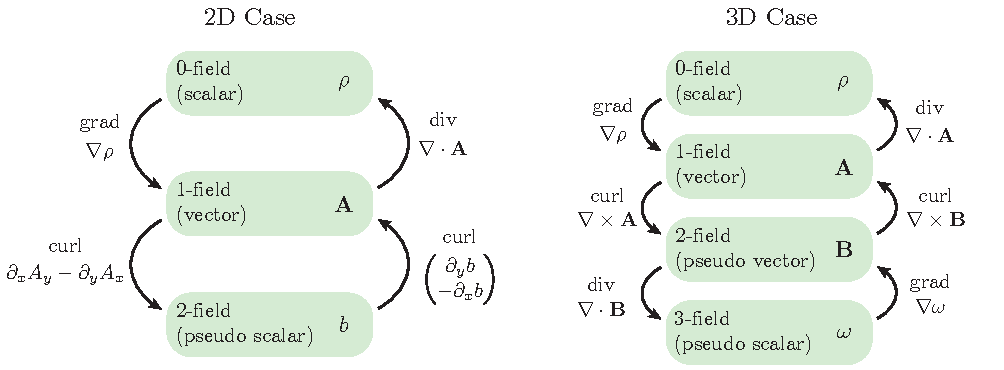
\includegraphics[width=1\linewidth]{figs/maps_to_forms.pdf}
    \caption{The different types of vector spaces that fields can live in for 2 and 3 dimensional systems. Differential operators can be used to create objects that live either in a higher or lower space, depending on what operator you use. }
    \label{fig:maps_to_forms}
\end{figure}


\section{Fradkin's Discretisation}
\begin{shaded}
    Fradkin's notation is a bit all over the place - since the intention of this section is to get a broad grip with what \cite{sun_fradkin_2015} does, our notation here will also be a bit of a mess. Fear not! in the next section it will be all clarified and made nice. 
\end{shaded}
Our starting point for Fradkin's lattice Chern-Simons theory is the `separate time and space' Lagrangian, which we re-express as 
\begin{align}
    \mathcal L = \frac{k}{2\pi}
    \left [  
    A_0  B -\frac 12 
    \textbf {A} \times \dot {\textbf {A}} 
    \right ].
\end{align}
Before we discretise this, let us check exactly what type of field each of the quantities presented here is,
\begin{center}
\begin{tabular}{|c|c|}
\hline
    $A_0$ & 0-form \\ 
    $\textbf A$ & 1-form \\ 
    $\nabla A_0$ & 1-form \\ 
    $B$ & 2-form \\ 
    \hline
\end{tabular}
\end{center}
Thus, the field splits into two parts, a scalar field 
\begin{align}
    A_0 \rightarrow a_j
\end{align}
and a vector field defined on edges
\begin{align}
    \textbf A \rightarrow A_{jk}, \textup{ with } A_{jk} = -A_{kj}
\end{align}
where in both the above definitions $j$ labels vertices on the lattice. Thus, there are four things we will need to define for the Hamiltonian to be translated into a lattice language:

\textbf{Gradient: } This is the simplest, where the gradient of a generic 1-form $\phi_j$ is written as a straightforward finite difference
\begin{align}
    (\nabla \phi)_{jk} = \phi_j - \phi_k
\end{align}
where this quantity is only nonzero if the lattice contains an edge $j \rightarrow k$. We can also index edges with $(jk)\rightarrow e$ and this can be labelled as $(\nabla \phi)_e$.

\textbf{Curl: } Again, the definition that they use is not terribly controversial, the curl of a vector field is defined as the sum of the field around a plaquette such that all fields are taken counter clockwise
\begin{align}
    (\nabla \times \textbf A)_f = \sum_{(jk) \in f} A_{jk},
\end{align}
where $f$ labels the face.

\textbf{Product between a 0-form and 2-form: }This is where things get weird. Unlike in the continuum, you cannot straghtforwardly take a product of $B$ and $A_0$, since one lives on faces and the other lives on vertices. Fradkin and co.~come up with an unforgivable solution to this problem. They assign a \textit{vertex-face correspondence} such that every vertex is adjacent to a face with which it is paired. In particular they do this by assigning a matrix $M_{vf}$ which is 1 for a paired edge and face and zero otherwise. This is needlessly complex. Rather we will just label vertices and faces with the same set of indices such that the $j$\ts{th} vertex is always paired with the $j$\ts{th} face. Thus, the first term in the Hamiltonian may be written as 
\begin{align}
    a_j B_j\textup{, with } B_j = \sum_{(jk) \in f} A_{jk},
\end{align}

\textbf{Cross Product: } Finally we get to the cross product, where their definition is so profoundly arbitrary and ugly that I shall not sully this document with it. Suffice to say they encode the cross product in a matrix $K_{e,e'}$, the construction of which can only be described as a crime against humanity. If you want to suffer like I did, read the paper, however the long and short of it is that the substitution they make for the second term in \ref{eqn:fradkin_starting_point} is 
\begin{align}
    \int d^2x \textbf {A} \times \dot {\textbf {A}} 
    \rightarrow 
    A_e K_{e,e'} \dot A_{e'}
\end{align}
where we have compressed each edge $(jk)$ with a single label $e$ to avoid $K$ having four subscripts...

Thus, we may write down the final action as 
\begin{align}
    S = \frac k{2\pi} \int dt \left [ 
    a_j B_j - \frac 12 A_e K_{ee'} \dot A_{e'}
    \right ]
\end{align}

\subsection{Gauge Symmetry}

Finally, let's discuss gauge invariance and then we'll move on to our more general formalism. Under a gauge transformation, we change the fields according to
\begin{align}
    a_j &\rightarrow a_j + \dot \chi_j\\
    A_{jk} &\rightarrow A_{jk} + \chi_j - \chi_k \qquad (=(\nabla \chi)_{jk})
\end{align}
Bearing in mind that the $B$-field term is invariant, the change to the action becomes
\begin{align}
    S \rightarrow S + \frac k{2\pi} \int dt
    \left [ 
        \dot \chi_j B_j 
        - \frac 12 (\nabla \chi)_e K_{ee'} \dot A_e
        - \frac 12 A_e K_{ee'} (\nabla \dot \chi)_e 
        - \frac 12 (\nabla \chi)_e K_{ee'} (\nabla \dot \chi)_e 
    \right ]
\end{align}
now let's use integration by parts to move the dot over on the second term here to get
\begin{align}
    S \rightarrow S + \frac k{2\pi} \int dt
    \left [ 
        \dot \chi_j B_j 
        -  \dot A_e K_{ee'} (\nabla \chi)_e 
        - \frac 12 (\nabla \chi)_e K_{ee'} (\nabla \dot \chi)_e 
    \right ]
\end{align}
This expression should really be understood as the discrete version of Eqn.~\ref{eqn:cont_intermediate_gauge} in the previous section. Now what we need is a discrete form of the Curl-Cross identity (Eqn.~\ref{id:curl_cross}). Let us start with the integral form of the identity for a pair of arbitrary fields u and $\textbf X$, where we have discarded the part that is a total derivative:
\begin{align}
\begin{matrix}
      \int d^2x 
      \left ( -\textbf{V} \times \nabla u   + u \nabla \times \textbf{V} \right ) = 0\\
    \downarrow \\
    - V_e K_{ee'} (\nabla u)_e + u_j (\nabla \times \textbf V)_j = 0
\end{matrix}
\end{align}
Now it may not be obvious but this is exactly the `gauge invariance' condition that Fradkin derive in Eqn.~4.5 of their paper. They go to great lengths to prove that this identity holds in general.

Finally a summary of the rest of Fradkin's paper. After spending a few pages proving that their cross product is a cross product and their curl is a curl, they go on to prove that the theory generally behaves like CS theory, with flux attachment. They also show that the theory is local (which wouldn't be necessary if they had used a better definition of the fields).

\section{Simplices, Boundaries and Products Done Right}

Let us now try and fix Fradkin's formalism, and come up with a much more general, less arbitrary way of doing the same thing. To do this we will follow the rather beautiful introduction to the relevant concepts from algebraic topology \cite{schwalm_vector_1999}. The discussion in their paper is complete, and very clear, so we will just poach the results that we want to extract, and leave the proofs/justifications to be found in the source material. 

The first thing to know is that their construction is defined specifically for a theory discretised on a \textit{simplicial complex}. Nakahara provides a nice introduction to simplices and their respective complexes \cite{nakahara_geometry_2003}, for the current project the only thing this means is that all plaquettes must be triangles. In practice this is not a terrible restriction, because we can always add edges to a given lattice to ensure that it satisfies this condition, as shown in Fig.~\ref{fig:simplices}a\footnote{Note that this is not a very unusual trick, see for example the triangulation used by Lieb in \cite{lieb_fluxes_2004}.}. 

\begin{figure}
    \centering
    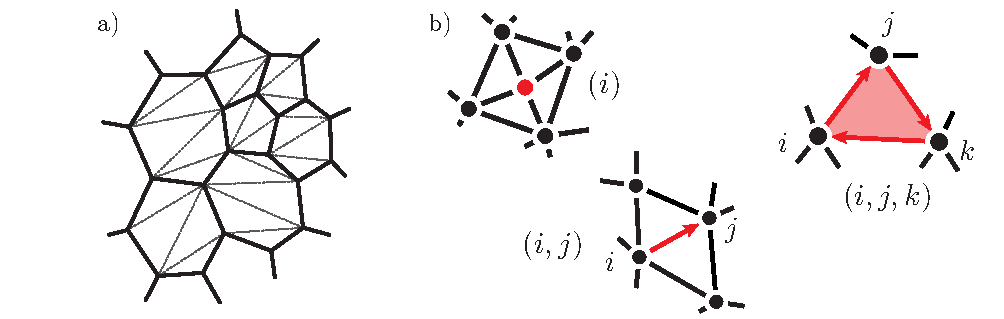
\includegraphics[width=1\linewidth]{figs/simplces.pdf}
    \caption{
    \textbf{(a)} Adding edges to a lattice to make it a simplicial complex.
    \textbf{(b)} An example of a 0,1 and 2-simplex.
    }
    \label{fig:simplices}
\end{figure}

Let us start by defining what a simplex is. A 0-simplex, denoted by $(i)$ is simply a vertex on the lattice, labelled at position $i$. To construct higher form simplices, we can add a vertex to a given simplex, provided that it is adjacent to all the vertices in that simplex. I.e.~$(i,j)$ is a 1-simplex which labels an edge from site $i$ to site $j$, whereas $(i,j,k)$ labels a triangle from $i$ to $j$ to $k$, as shown in Fig.~\ref{fig:simplices}b. Note that all simplices have the property that they are antisymmetric under permutation of thier indices. That is, for a general permutation $\mathcal P$
\begin{align}
    (P(j), P(j), P(k), ..., P(n)) = \textup{sgn}(P) (i,j,k,...,n).
\end{align}

Now we can use the set of all $n$-simplices as a basis for constructing fields! Here we define an $n$-field as an element of the vector space spanned by all $n$-simplices:
\begin{align}
    \textup{0-form: } \phi &= \sum_{[i]} (i) \phi_{i}  \\ 
    \textup{1-form: } \alpha &= \sum_{[i,j]} (i,j) \alpha_{ij} \\ 
    \textup{2-form: } \beta &= \sum_{[i,j,k]}(i,j,k) \beta_{ijk} 
\end{align}
where the general field term must always be antisymmetric under permutation of the indices, eg:
\begin{align}
    \beta_{ijk} = - \beta{jik}
\end{align}

\begin{shaded}
    It might make sense to include a factor of $\frac 1{n!}$ in the field term of a general $n$-form... This would line up nicely with the continuous theory of differential forms. Let's see later if we want to introduce it.
\end{shaded}

\subsection{Derivative Operators}

Now let us define a notion of `differentiation' on these fields. There are two derivative operators that we will introduce, parachuted in directly from the mathematics of differential forms: the boundary $\partial$ and the coboundary $d$. These operators act directly on the simplices, and effectively ignore the field degree of freedom. In essence, when acted on a generic $n$-field $\gamma$
\begin{align}
    \partial \gamma = \partial \sum_{[i,j,k,...,n]} \gamma_{ijk...n} \partial (i,j,k,...,n),
\end{align}
with the same property for $d$.

\begin{figure}
    \centering
    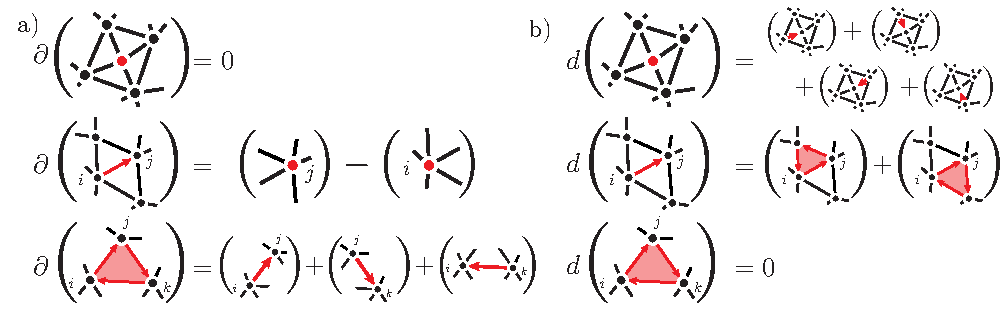
\includegraphics[width=\linewidth]{figs/boundaries.pdf}
    \caption{
    \textbf{(a)} The action of the boundary operator on a general 0, 1 and 2-simplex.
    \textbf{(b)} The action of the coboundary operator on a the same set of simplices.
    }
    \label{fig:boundaries}
\end{figure}
\subsubsection{Boundary}
The boundary is a map from $n$-simplices to $(n-1)$-simplices. The operation is simple, 
\begin{align}
    \partial (i,j,k,l,...) = (j,k,l,...) - (i,k,l,...) + (i,j,l,...) - (i,j,k,...) + ...
\end{align}
That is, we form a sum of every simplex formed by dropping one vertex, with the sign determined by whether the position of the deleted vertex is odd or even. Let us calculate a few examples, which are shown visually in Fig.~\ref{fig:boundaries},
\begin{align}
    \partial (i) &= 0, \\
    \partial (i,j) &= (j) - (i), \\
    \partial (i,j,k) &= (j,k) - (i,k) + (i,j).
\end{align}
We can also calculate the effect of this operator on our fields. Firstly, it can be seen that the boundary acting on a 0-field always vanishes,
\begin{align}
    \partial \phi & = 0.
\end{align}
Next, the boundary of a 1-field is given by
\begin{align}
    \partial \alpha & = \sum_{[i,j]}
    \left [ 
    (j) - (i)
    \right ]
    \alpha_{ij} , \\
    & = \sum_{[i]} (i) \sum_{[j] \rightarrow [i]}
    \alpha_{ji},
\end{align}
where the second sum is over all vertices $j$ adjacent to $i$. This is rather promising -- if you picture $\alpha_{ij}$ as something like a current (or electric field) then this would tell you how much current is entering or exiting site $i$ from its neighbours! I.e.~this looks a lot like a divergence! Let us carry on by calculating the case for a 2-field,
\begin{align}
    \partial \beta &= \sum_{[i,j,k]} 
    \left [
    (j,k) - (i,k) + (i,j)
    \right ]
    \beta_{ijk} \\
    & = \sum_{[i,j])} (i,j) 
    \sum_{[k]\rightarrow [i,j]}
    \beta_{ijk},
\end{align}
where the second sum is over all vertices $k$ that are adjacent to \textit{both} $i$ and $j$. This is even more promising! Imagining $\beta$ as a quantity like vorticity, this calculates exactly the current that would be generated on the edge $(i,j)$ as a consequence of difference in vorticity in the two adjacent triangles. I.e. this looks a lot like a curl!

\begin{figure}
    \centering
    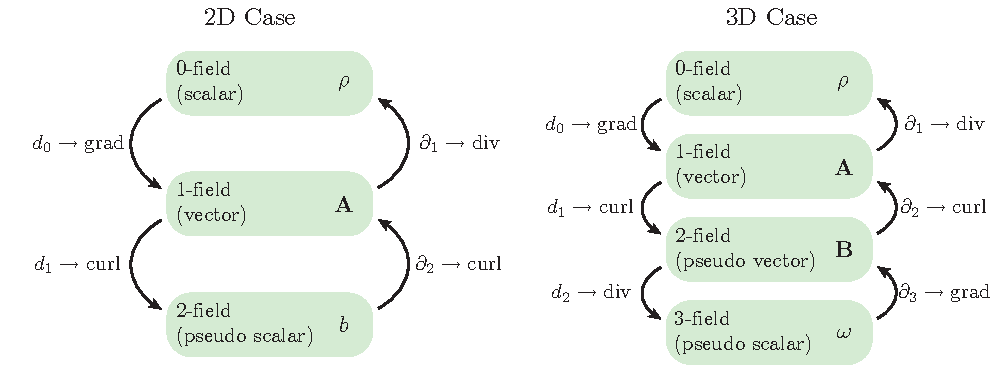
\includegraphics[width=\linewidth]{figs/maps_to_forms_boundaries.pdf}
    \caption{We repeat the hierarchy of operations depicted in Fig.~\ref{fig:maps_to_forms}, now showing the action of the boundary and coboundary operators.}
    \label{fig:maps_to_forms_boundaries}
\end{figure}



\subsubsection{Coboundary}

Now we turn our attention to the coboundary operator $d$, which is defined as 
\begin{align}
    d(i,j,k,...,n) = \sum_{[u]\rightarrow [i,j,k,...,n]}(u,i,j,k,...,n).
\end{align}
Let's again play the game of seeing how this operator acts on our fields. Lets start with a 0-field
\begin{align}
    d\phi &= \sum_{[j]} \sum_{[i]\rightarrow [j]} \phi_j (i,j) \\
    & = \sum_{[i,j]}(\phi_j - \phi_i) (i,j)
\end{align}
As before, we might notice that this operator acts a bit like a discrete version of the grad operator! Now looking at 1-fields we find that
\begin{align}
    d\alpha &= \sum_{[j,k]} \sum_{[i]\rightarrow [j,k]} \alpha_{jk} (i,j,k), \\
    & = \sum_{[i,j,k]}(\alpha_{ij} - \alpha_{ik} + \alpha_{jk}) (i,j,k)
\end{align}
Again, treating $\alpha_{jk}$ as a current this looks a lot like a curl operator! In fact, by considering Fig.~\ref{fig:maps_to_forms} we can see that the boundary and coboundary operators correspond exactly to the differential operators that can map continuous fields between the different `levels'.

\subsubsection{Inner Product and Stokes Theorem}

To complete this discussion of our discrete calculus, we must also define a discrete analog of integration. To do this let us introduce an ordered $n$-chain $\mathcal C$ as the discrete analog of an oriented arc or surface. Chains are also organised into a hierarchy of $n$-forms
\begin{align}
    \mathcal C_0 &= \sum_{[i]\in \mathcal C} (i), \\
    \mathcal C_1 &= \sum_{[i,j]\in \mathcal C} (i,j), \\
    \mathcal C_2 &= \sum_{[i,j,k]\in \mathcal C} (i,j,k).
\end{align}
We must also define an inner product on forms, given by
\begin{align}
    \inner{(i)(l)} & = \delta_{i,l},\\
    \inner{(i,j)(l,m)} & = \delta_{i,l}\delta_{j,m} -\delta_{i,m}\delta_{j,l}.
\end{align}
for a general $m$-form the inner product is given by
\begin{align}
    \inner{(i,j,k,...)}{(l,m,n,...)} = \textup{det}\begin{pmatrix}
        \delta_{il} & \delta_{im} & \delta_{in}\\
        \delta_{jl} & \delta_{jm} & \delta_{jn}& \cdots\\
        \delta_{ikl} & \delta_{ikm} & \delta_{kn}\\
        & \vdots & & \ddots
    \end{pmatrix}.
\end{align}
This looks really complicated but it actually isn't. All we're saying is that the product is only nonzero if $(i,j,k,...)$ and $(l,m,n,...)$ contain exactly the same vertices as one another, but if they are ordered differently then we might pick up a factor of $-1$ from reordering the indices to make the two forms identical. 

Now we can define the analog of a line intergal, as the inner product of a 1-chain and a 1-field:
\begin{align}
    \inner {\alpha, C} = \sum_{[i,j]\in C} \alpha_{ij}.
\end{align}
Now look at 
\begin{align}
    \inner {d\phi, C} &= \sum_{[i,j]\in C}(\phi_j - \phi_i),\\
    & = \phi_b - \phi_a.
\end{align}
where vertex $b$ is where the chain ends and $a$ is where the chain starts. Thus, we can see immediately that
\begin{align}
    \inner {d \phi, C} = \inner {\phi, \partial C}
\end{align}
In fact, this expression holds for any general pair consisting of a $n$-form $\xi$ and an $(n+1)$-form $\zeta$
\begin{align}
    \inner {d\xi, \zeta} = \inner {\xi, \partial \zeta}
\end{align}
and we have the discrete form of Stokes' law, in a completely elegant form.

\subsection{Products}

\begin{shaded}
    I'll fill this in properly later -- there has to be a much nicer and more general picture than what is in the paper \cite{schwalm_vector_1999} where they derive slowly and painfully the correct version of each type of product such that the theory respects the standard set of vector calculus identities. I think there is a more general perspective where these different expressions should all look obvious (i.e.~we want to find the generalisation of the exterior product from diff.~forms to these simplices) for now let's just stick the relevant identities in and move on with the Chern Simons stuff. Later on I will come back and figure out how to do this.
\end{shaded}

\subsubsection{Scalar Multiplication}


Scalar multiplication basically amounts to taking a product between a 0-form and a (something else)-form. Let's put down the general identities for the product between a 0-form $\phi$ and an $n$-form $\xi$,
\begin{align}\begin{aligned}
    \phi \xi &= 
    \left (
    \sum_{[i] } \phi_i (i)
    \right )
    \left (
    \sum_{[i,j,k,...,m] }\xi_{ijk...m} (i,j,k,...,m)
    \right ) \\
    &=\sum_{[i,j,k,...,m]}
    \frac 1n (\phi_i + \phi_j + \phi_k + ... + \phi_m)
    \xi_{ijk...m} (i,j,k,...,m)
\end{aligned}
\end{align}
Basically what is happening here is that each vertex that touches the $n$-form contributes $\frac 1n$ of its field value to the product. 



\subsubsection{Dot Products}
\begin{shaded}
    We don't actually need these yet...
\end{shaded}

\subsubsection{Cross Products}

A cross product of two 1-forms creates a 2-form. We will define the cross product between two 1-fields $\alpha$ and $\sigma$ as 
\begin{align}
    \alpha \times \sigma = 
    \sum_{[i,j,k]} \frac 16 \left [ 
    (\alpha_{ki} +\alpha_{kj} )\sigma_{ij}
    + (\alpha_{ij} +\alpha_{ik} )\sigma_{jk}
    + (\alpha_{ji} +\alpha_{jk} )\sigma_{ki}
    \right ](i,j,k)
\end{align}
\begin{shaded}
    This is all we really need for Chern Simons Theory, although it would be really nice to have a more complete framework where products felt more natural...
\end{shaded}

\section{Chern Simons on Any Lattice}

Now let us apply the developed discretisation procedure to create  a lattice Chern Simons theory. We start as ever by restating the continuous-space action
\begin{align}
    S = \frac{k}{2\pi}
    \int dt \int d^2x
    \left [  
    A_0  B -
    \textbf {A} \times \dot {\textbf {A}} -
    \nabla A_0  \times  \textbf {A}
    \right ].
\end{align}
Let us make our substitutions for the simplicial versions of these fields:
\begin{align}
    A_0 \rightarrow \rho = \sum_{[i]}\rho_i(i),\\
    \textbf A \rightarrow \alpha = \sum_{[i,j]}\alpha_{ij} (i,j).
\end{align}
Next, we can calculate the two derivative forms in the expression
\begin{align}
    \nabla A_0 \rightarrow d\rho &= \sum_{[i,j]}(\rho_j - \rho_i) (i,j),\\
    B \rightarrow d\alpha  &= \sum_{[i,j,k]} ( \alpha_{ij} + \alpha_{jk} + \alpha_{ki}) (i,j,k)
\end{align}
Therefore we can write the integrand in the form
\begin{align}
    \rho d\alpha - \alpha \times \dot \alpha + \alpha 
    \times d\rho. 
\end{align}
Defining a 2-chain that covers the whole complex (i.e. all of space),
\begin{align}
    C = \sum_{[i,j,k]} (i,j,k)
\end{align}
we can write the action in the form
\begin{align}
    S = \frac k{2\pi} \int dt \inner{C, 
    \rho d\alpha 
    - \alpha \times \dot \alpha 
    -  d\rho \times \alpha
    }
\end{align}
\begin{shaded}
    {\it Single mom finds one weird vector identity for simplifyinf equations FAST --- } There is only one vector identity that is really relevant to this action, and it is the same one we used in \textsection{\ref{sec:continuous_special_time}}:
    \begin{align} 
            \nabla \times (a \textbf{A}) = \nabla a \times \textbf{A} + a \nabla \times \textbf{A},
        \end{align}
        where $a$ is a scalar and $\textbf A$ is a 1-field. Let us derive the simplicial equivalent of this expression
        \begin{align}
            d(\rho \alpha) = \sum_{[i,j]}\frac 12 (\rho_i + \rho_j) \alpha_{ij} d(i,j),
        \end{align}
        where we have used the definition presented above for 0-1-form multiplication. Taking the coboundary of (i,j) we arrive at the following
        \begin{align}
             d(\rho \alpha) &= \sum_{[i,j,k]}\frac 12 
             \left [
             (\rho_i + \rho_j)\alpha_{ij}
             + (\rho_j + \rho_k)\alpha_{jk}
             +(\rho_k + \rho_i)\alpha_{ki}
             \right ]
        \end{align}
    which is rearranged to the form
    \begin{align}
        \begin{aligned}
            d(\rho \alpha) &= \sum_{[i,j,k]} \frac 13 (\phi_i + \phi_j +\phi_k)(\alpha_{ij} + \alpha_{jk}+\alpha_{ki}) \\ 
            &
            + \sum_{[i,j,k]} \frac 16 \bigg [
            [(\phi_i - \phi_k) + (\phi_j - \phi_k)]\alpha_{ij}
            + [(\phi_j - \phi_i) + (\phi_k - \phi_i)]\alpha_{jk}\\& \qquad \qquad 
            + [(\phi_k - \phi_j) + (\phi_i - \phi_j)]\alpha_{ki}
            \bigg ] (i,j,k)
        \end{aligned}
    \end{align}
    This looks like a mess, but consulting our earlier identities for cross and scalar product, we can actually see that this exactly evaluates
    \begin{align}
        d(\rho \alpha) = \rho d\alpha + d\phi \times \alpha.
    \end{align}
\end{shaded}

\subsection{Gauge Transformations}

\bibliography{refs}
\end{document}
